% 本文件是示例论文的一部分
% 论文的主文件位于上级目录的 `bachelor.tex` 或 `master.tex`

\chapter{工作}

\section{公平性研究}
公平性问题是指,不同车辆通过同一个路口的通行时间可能有很大的差别,因为信号灯可能为了提高整体通行效率而牺牲一些车辆,让这些车辆多等待一些时间,即便这些车辆可能是先进入路口的,这对这些车来说是不公平的。一个好的控制策略应该在提高通行效率的同时能够保证每辆车所需的通行时间大致相同,也就是说,车辆通行时间的方差应该越小越好。但是已有的工作都是使用车辆的平均通行时间来衡量通行效率,很自然的忽略了公平性问题。
\subsection{目标}
本工作的目的是在提高通行效率(最小化平均通行时间)的同时,希望每条车道能够有尽可能相同的服务延迟(得到放行所需的时间)。这个目标可以用以下的Jain Fairness Index(JFI)指标来量化:
\begin{align}
    \mathcal{J} = \frac{(\sum_{i=1}^{M}\overline{D}_i)^2}{M\sum_{i=1}^{M}\overline{D}_i^2},
\end{align}
其中$\overline{D}_i$是第$i$条进近车道的平均延迟。当且仅当每一个$\overline{D}_i$都相等时,这个指标达到最大值,即是$1$。所以我们的目标也就是最大化这个指标。

\subsection{智能体设计}
\subsection*{状态表示}
在$t$时刻的状态$S(t)$由以下几个部分组成:
\begin{enumerate}
\item 交通流量:$\boldsymbol{V}(t)=\{V_1(t),V_2(t),\cdots,V_M(t)\}$。其中 $V_i(t)$表示第$i$条进近车道上车的数量。值得注意的是,由于右转不受限于信号灯的特殊性,这里我们不考虑右车道的交通流量。
\item 平均吞吐量:$\boldsymbol{\overline{L}}(t)=\{\overline{L}_1(t),\overline{L}_2(t),\cdots,\overline{L}_M(t)\}$。其中$\overline{L}_i(t)$表示第$i$条进近车道的平均吞吐量。同上,不考虑右车道的平均吞吐量。
\item 信号相位:$\boldsymbol{P}(t)$是当前信号相位的数字化表示,$1$表示绿色,可以通行;$0$表示红色,禁止通行。
\end{enumerate}
所以$S(t)=\{\boldsymbol{V}(t) || \boldsymbol{\overline{L}}(t) || \boldsymbol{P}(t) \}$
\subsection*{动作选择}
在本文中,动作选择机制是每次选择即将转换的信号相位。之后,交通信号灯将转换到这一新的相位并持续$\Delta t$的时间。为了安全起见,我们在两个不同的信号相位之间插入了3秒的黄色信号和2秒的红色信号。如果新选择的相位和当前相位相同,则不插入黄色和红色信号,以确保交通流畅。
\subsection*{奖励函数}
受PFS分配原则的启发,我们设计了一个可以在效率和公平之间提供良好的平衡的奖励函数,如下所示:
\begin{align}
\label{eq:reward}
    r = -\sum_{i=1}^{M} \frac{Q_i(t)}{\overline{L}_i(t) + \delta},
\end{align}
其中$Q_i(t)$ 和 $\overline{L}_i(t)$ 分别是第$i$条进近车道的队列长度和平均吞吐量。在每一次调度后(这里,我们将一次动作选择视作一次调度),$\overline{L}_i(t)$ 按照以下方式进行更新:
\begin{align}
    \overline{L}_i(t) = (1-\frac{1}{W})\overline{L}_i(t-1) + \frac{1}{W}L_i(t),
\end{align}
其中$L_i(t)$是此次调度中车道$i$上得到放行的车的数量,$W$是一个平衡通行效率和公平性的参数。另外,为了避免公式\ref{eq:reward}的分母为0, 我们加上了一个可以忽略不计的正数$\delta$。
\subsection*{训练过程}
训练过程伪代码如下:

\section{通信问题研究}
对于多路口的交通信号调度问题,协作(Coordination)可以有效地提升整体通行效率,以下列出几种常见的协作策略:
\begin{table}[htb]
    \caption[协作策略]{常见的协作策略\label{tab:coordination}}
    \begin{tabular}{clp{0.4\columnwidth}}
      \toprule
      协作策略 & 目标 & 说明 \\
      \midrule
      Global single agent & $max_{\mathbf{a}}Q(s, \mathbf{a})$ & $s$是全局的环境状态,$\mathbf{a}$是所有路口的联合动作。\\
      Independent RL without Communication & $max_{a_{i}}\sum{i}Q_{i}(o_i, a_i)$ & $o_i$是路口$i$的局部观测,$a_i$是路口$i$的动作。\\
      Independent RL with Communication & $max_{a_i}\sum{i}Q_i(\Omega(o_i, \mathcal{N}_i), a_i)$ &$\mathcal{N}_i$是路口$i$的邻近路口的状态表示,$\Omega(o_i, \mathcal{N}_i)$是整合路口$i$及其邻近路口状态表示的函数。\\
      \bottomrule
    \end{tabular}
\end{table}


使用GAT来学习communication,这样做有一下两个好处:
1. 动态学习周边的路口的重要性:已有的工作直接将目标路口及其邻近路口的状态直接整合起来,这种做法实际上是默认每一个邻近路口对目标路口的影响力是相同的。实际上由于交通在时间和空间上的变化,
同一个路口对于其目标路口的影响力也会发生变化。
2. 免索性模型学习(Index-free modeling learning):在多智能体场景下,通常需要使用参数共享(Parameter Sharing)来降低学习难度,从而加速学习。但是这一点在多路口信号控制场景下是不适用的,
因为不同路口对其邻近路口的敏感性是不同的。例如,如下图所示,有A,B两个路口,A对其N-S方向的交通更加敏感,B对其W-E方向的交通更加敏感,如果直接将A的参数分享给B,会导致B学习到的策略并不适用于
自身的场景。
\begin{figure}[htb]
  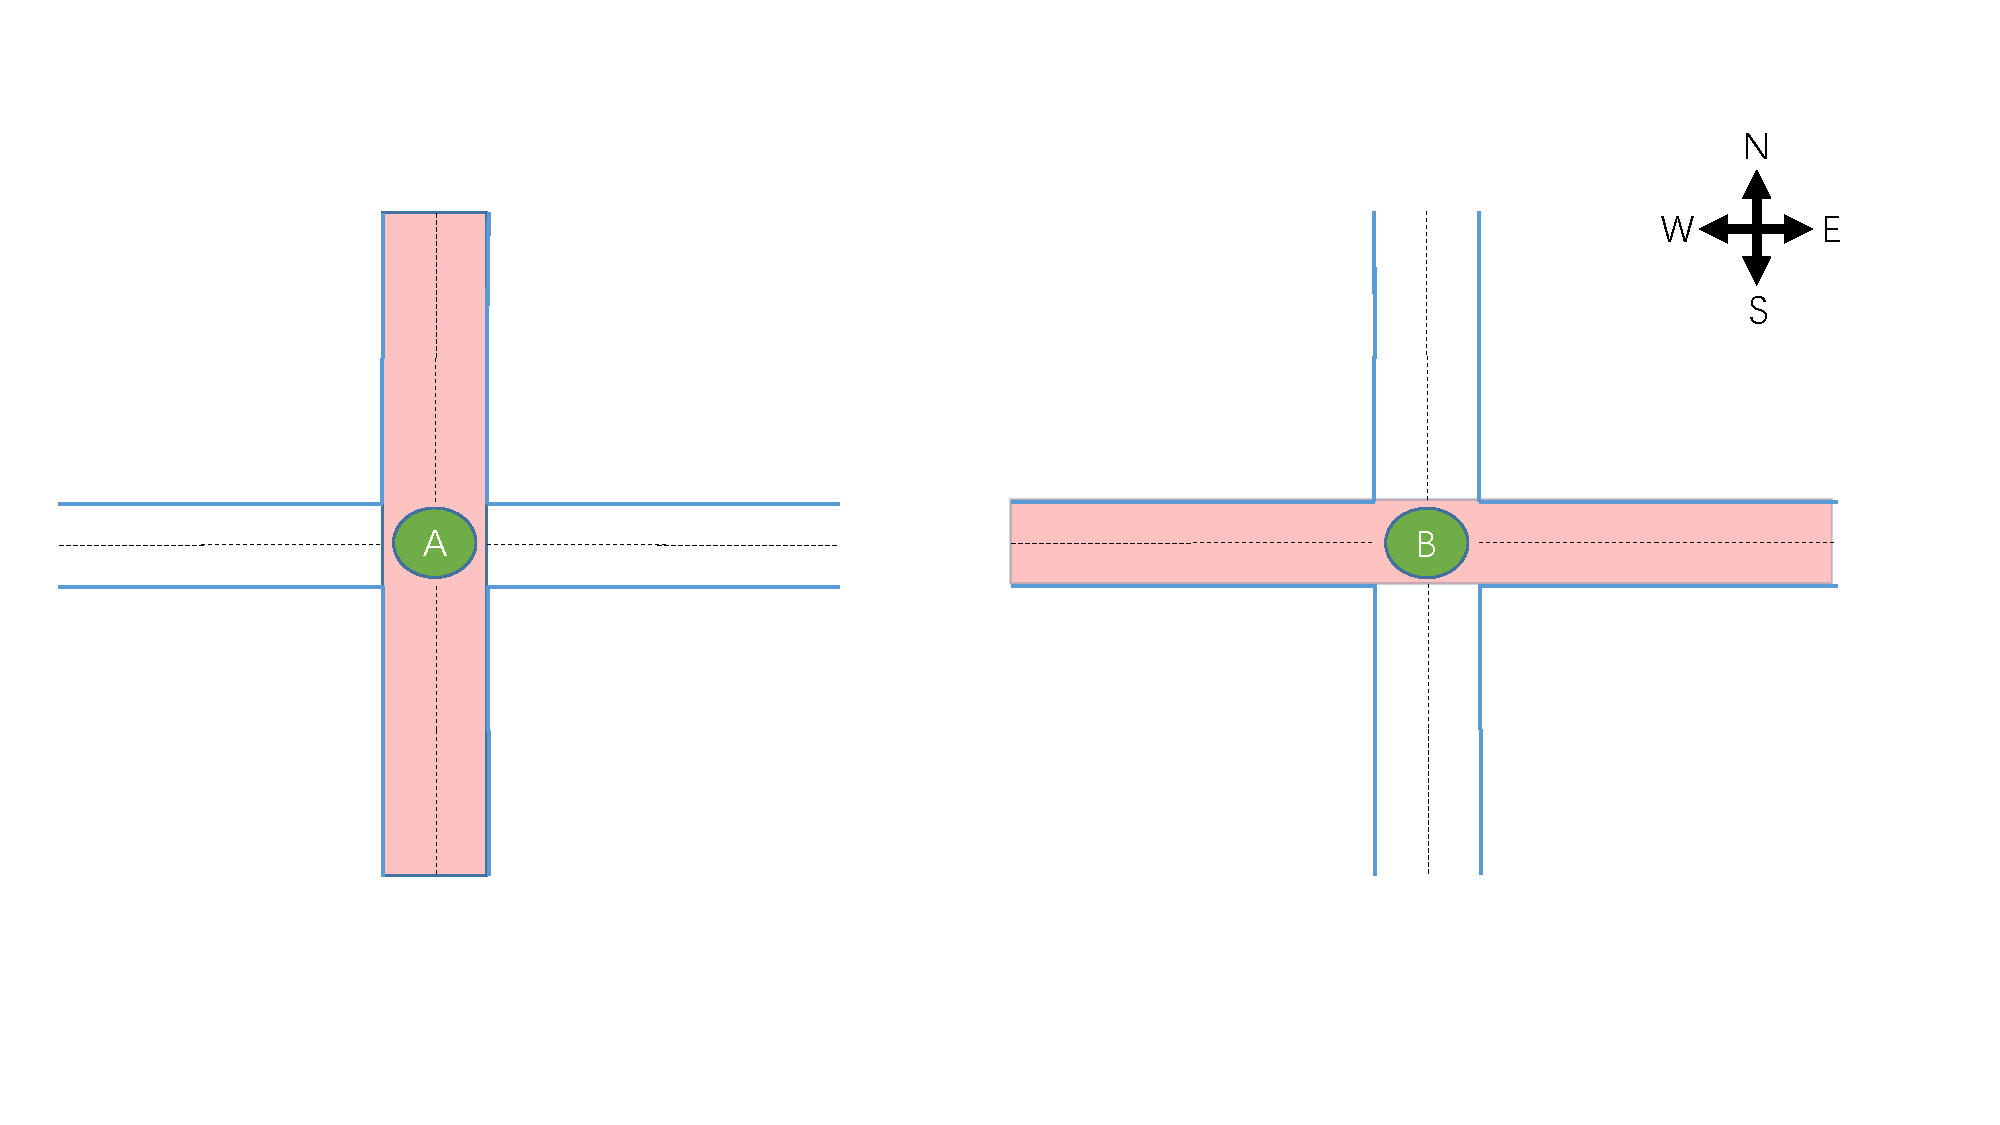
\includegraphics[width=10cm]{ppt/index-free.pdf}
  \caption{路口敏感性说明}
  \label{fig:index-free}
\end{figure}

使用IRL with communication的方法确实可以有效的解决维度灾难的问题。
已有的工作使用图神经网络来学习“交流”这一个过程。他们将每一个路口视作图中的一个节点,每条道路作为连接两个节点的边,很自然地可以将一张交通道路网建模成一个图。这种按路口建模的方式如下所示:
\begin{figure}[htb]
  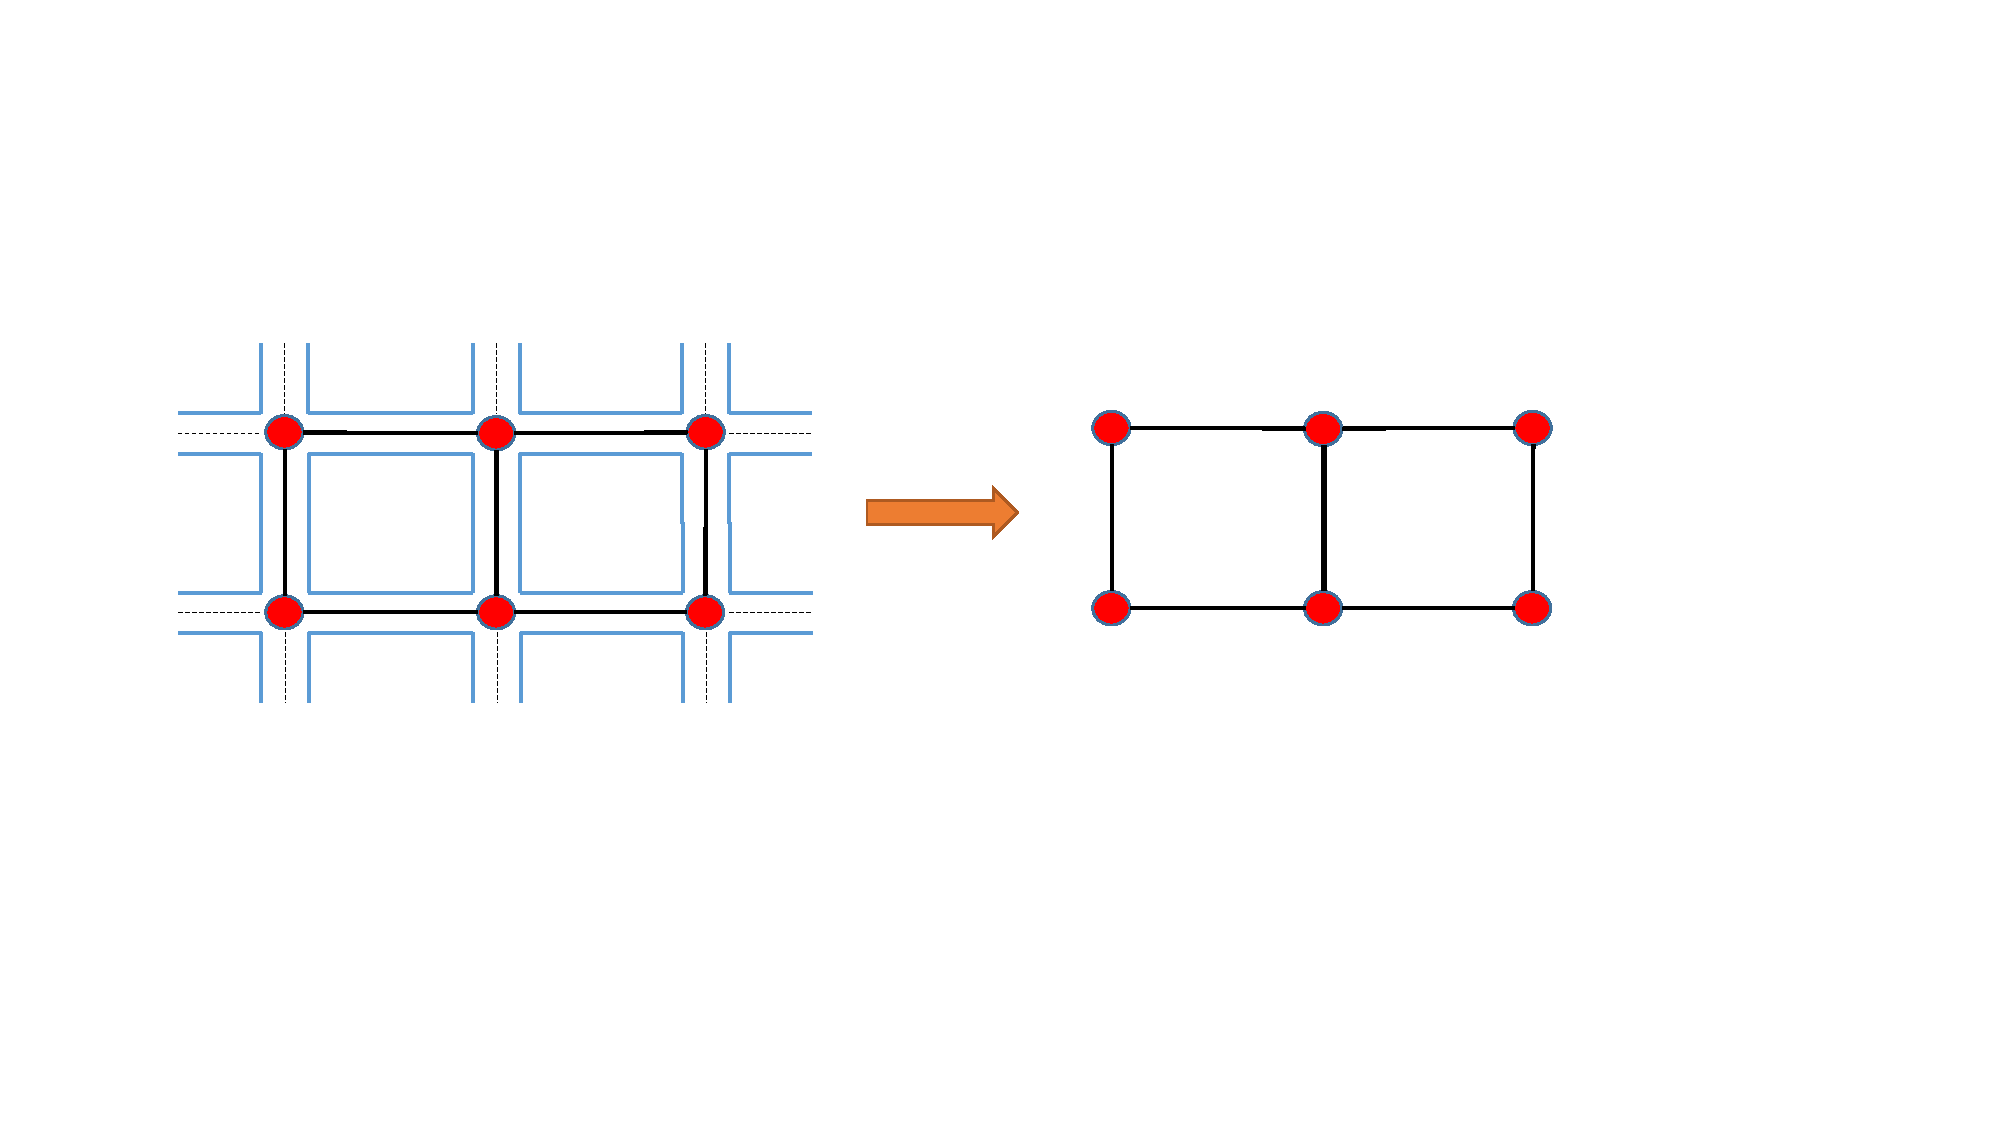
\includegraphics[width=10cm]{ppt/network-graph.pdf}
  \caption{多路口建模成图(路口)}
  \label{fig:network-graph-old}
\end{figure}

在这种建模方式下,每条车道的车辆以及当前的相位将作为该节点的特征。这种建模方式虽然可以很清晰的将多路口场景变成一张图。但是,因为是以一个路口为一个节点,所有车道的状态信息都整合到了一起,有些车道的的信息对目标节点是无用的,
如下图所示:
\begin{figure}[htb]
  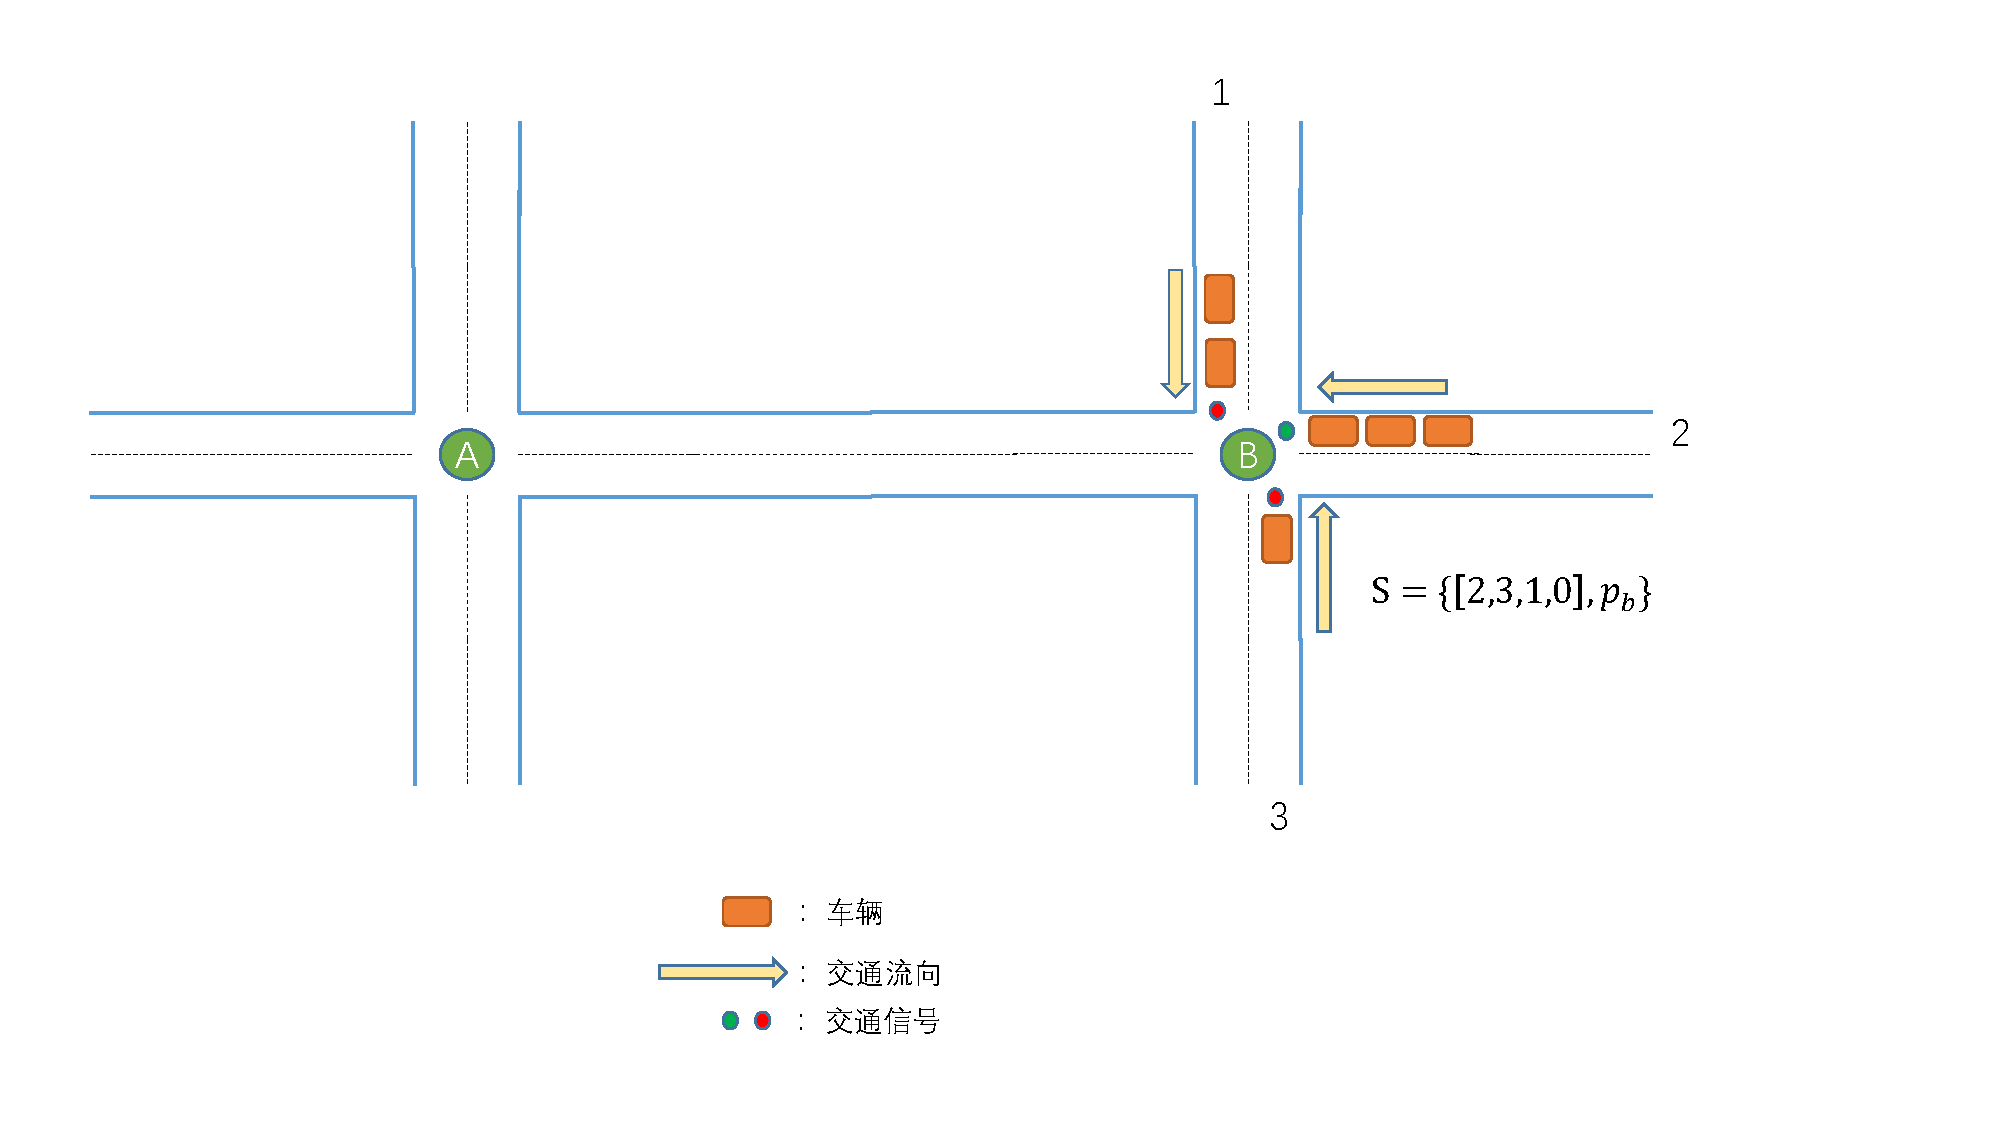
\includegraphics[width=12cm]{ppt/information-redundancy.pdf}
  \caption{按路口建图模式下信息传递}
  \label{fig:information-redundancy}
\end{figure}

路口B中只有2车道的交通流向与A车道有关,1、3车道的车辆不会行驶到A路口。在信息传递的时候,如果将所有的信息都笼统地传递过去,将会增加A提取有效信息的难度,从而降低学习的效率。

此外


在本文中,我们采用GAT来学习communication,不同的时,我们采用不同的图建模方式。我们不是按照路口来建图,而是按照道路来进行建模,即一条道路就是一个节点,如下图所示:
\begin{figure}[htb]
  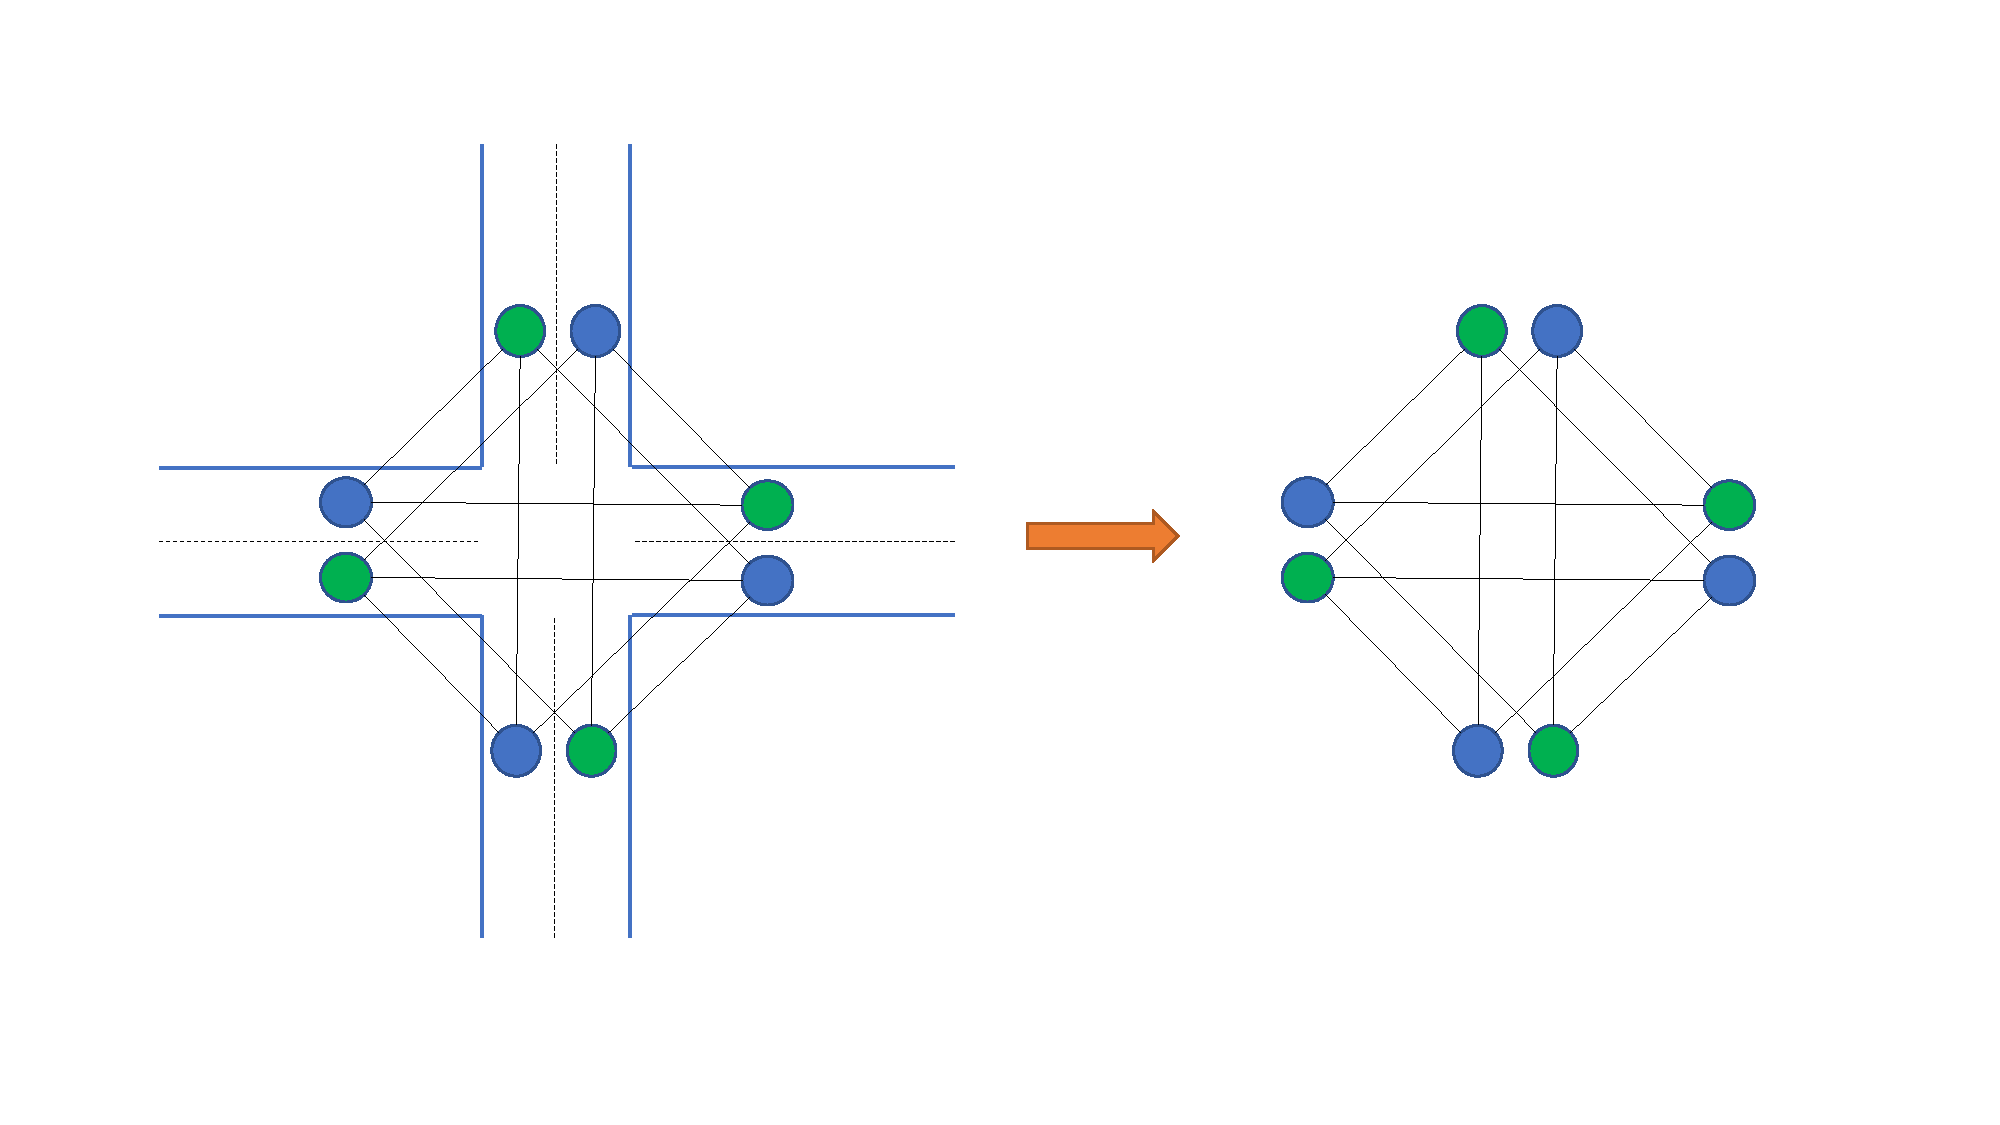
\includegraphics[width=12cm]{ppt/graph-modeling.pdf}
  \caption{按道路建模成图}
  \label{fig:network-graph-new}
\end{figure}
两个好处:1,减少无关信息的传递;2,将相位由数字化特征变成结构化特征。

